\documentclass[11pt,a4paper]{article}
\usepackage[T1]{fontenc}
\usepackage[utf8]{inputenc}
\usepackage{lmodern,microtype}
\usepackage{amsmath,amssymb,amsthm,mathtools,bm}
\usepackage{booktabs,array,tabularx,longtable}
\usepackage{graphicx,float,caption}
\usepackage{xcolor}
\usepackage[margin=20mm]{geometry}
\usepackage{enumitem}
\usepackage{fancyhdr}
\usepackage[hidelinks]{hyperref}
\hypersetup{
  pdftitle={FIN ST01--ST15: Shadow-to-Physics Bridge Research},
  pdfauthor={Krzysztof Żuchowski},
  pdfsubject={Local analytical and computational execution of programs ST01--ST15},
  pdfkeywords={FIN, spectral operator, physical shadow, continuum, gauge, thermodynamics, Krein theory, renormalization}
}
\setlength{\parindent}{0pt}
\setlength{\parskip}{0.50em}
\setlength{\emergencystretch}{2em}
\setlength{\headheight}{14pt}
\setlist[itemize]{leftmargin=1.55em,itemsep=0.16em,topsep=0.2em}
\setlist[enumerate]{leftmargin=1.75em,itemsep=0.16em,topsep=0.2em}
\pagestyle{fancy}
\fancyhf{}
\lhead{FIN ST01--ST15}
\rhead{Release 10.55}
\cfoot{\thepage}
\newtheorem{theorem}{Theorem}[section]
\newtheorem{proposition}[theorem]{Proposition}
\newtheorem{corollary}[theorem]{Corollary}
\newcommand{\proven}{\textcolor{green!40!black}{\textbf{[PROVEN]}}}
\newcommand{\strong}{\textcolor{blue!70!black}{\textbf{[STRONG EVIDENCE]}}}
\newcommand{\conditional}{\textcolor{black!60}{\textbf{[CONDITIONAL]}}}
\newcommand{\failed}{\textcolor{red!72!black}{\textbf{[FAILED/OPEN]}}}
\newcommand{\boundary}{\textcolor{orange!80!black}{\textbf{[BOUNDARY]}}}
\newcommand{\resultbox}[1]{\begin{center}\fcolorbox{blue!60!black}{blue!4}{\parbox{0.92\textwidth}{#1}}\end{center}}

\begin{document}

\pagenumbering{gobble}
\begin{titlepage}
\centering
\vspace*{1.55cm}
{\LARGE\bfseries FIN ST01--ST15\par}
\vspace{0.38cm}
{\Large Shadow-to-Physics Bridge Research\par}
\vspace{0.45cm}
{\large Exact theorems, null controls, conditional constructions, and obstruction results for the current finite FIN operator framework\par}
\vspace{1.25cm}
{\Large Krzysztof Żuchowski\par}
\vspace{0.24cm}
{\large Independent Researcher --- Fractal Information Theory Project\par}
{\large ORCID: 0009-0002-0909-3613\par}
\vspace{1.05cm}
{\large FIN Release 10.55 --- Version 1.0.0\par}
{\large August 10, 2026\par}
\vfill
\begin{minipage}{0.88\textwidth}
\textbf{Research premise.} The report executes the fifteen local programs proposed by Release 10.54. It does not assume that FIN is a Theory of Everything. The FIN-as-ToE statement remains a counterfactual organizing hypothesis.\par
\textbf{Method.} All results are analytical, symbolic, or numerical and were generated locally. Five null classes, $6{,}000$ sampled operators, a separate $5{,}000$-sample frozen holdout, exact symbolic identities, negative controls, and seventeen regression tests are included.\par
\textbf{Epistemic rule.} Exact matrix identities are not called physical derivations. Constructed mediators, link phases, labels, scales, baths, and refinements remain explicit additional premises.\par
\textbf{Repository.} \url{https://github.com/hyconiek/Fractal-Nadsoliton-Theory}\par
\textbf{License.} CC BY 4.0.
\end{minipage}
\end{titlepage}
\pagenumbering{arabic}

\begin{abstract}
This report executes Programs ST01--ST15 against the frozen strict FIN operator
\[
W_{xx}=0,\qquad W_{xy}=K_{\rm strict}(d(x,y))\quad(x\ne y),\qquad
A=sI-W\succeq0
\]
on $C_{12}$. The work asks whether the exact common spectral calculus of $A$ can be promoted into a physical reduction without silently inserting the missing structures.

The answer is mixed. ST01 gives a typed physical-shadow certificate and proves the composition law for approximate reductions. ST02 reconstructs one generator from unitary, heat, Green, Gibbs, and wave channels with relative errors below $4.3\times10^{-15}$; a $2.39\%$ altered-generator channel and an aliased unitary control are rejected. ST03 shows that isospectral rotations preserve the spectrum to $4.9\times10^{-15}$ while destroying the FIN vertex geometry and Markov property. Thus spectrum alone cannot identify the substrate. ST04 proves that one additional distinct diagonal vertex observable enlarges $C^*(A)$ from dimension $7$ to $M_{12}(\mathbb C)$ of dimension $144$, but the observable imports labels and orientation. An unoriented anchored observable reaches only dimension $74$, while a chiral circulant reaches $12$.

ST05 constructs two equally valid continuations agreeing at $N=12$ but having gap exponents approximately $-1.965$ and $-0.086$. The direct integer-distance continuation first becomes signed at distance $8$ and loses the Markov property. Hence the present endpoint does not select a canonical continuum family. ST06 proves that the all-distance strict kernel has no nontrivial exact cyclic causal cone: every remote vertex receives a first-order unitary and heat tail and a second-order wave tail.

ST07 proves the relative-entropy/free-energy bridge once a state, Hamiltonian, bath temperature, process class, and energy unit are supplied; the bridge does not source those objects. ST08 constructs a gauge-covariant $U(1)$ link model with covariance, holonomy, and continuity residuals below $7\times10^{-16}$, but the connection and group are inserted. ST09 constructs a globally coercive saturating mediator with the required attractive fourth-order jet. Its saturation scale and positive coercive term are new axioms. ST10 verifies the Hamiltonian $J_0L$ memory structure exactly in the implemented blocks and locates a numerical transition in mediator speed within $[1.24,1.28]$, but an exact Krein certificate remains open.

ST11 proves exact Schur-elimination associativity to $3.5\times10^{-16}$ and shows that a declared truncation produces a $0.782\%$ scheme difference; this is not yet an RG fixed point. ST12 blocks all legacy physical-role transfer because completion and role-invariance theorems remain absent. ST13 validates a heat-calibrated, no-refit synthetic cross-channel pipeline and rejects an altered unitary holdout. ST14 preregisters and hashes a kernel fingerprint before a $5{,}000$-sample holdout; it has zero false accepts, but is rejected as a physical prediction because it restates the defining kernel formula. ST15 passes six symbolic, rational, and numerical core checks with an explicit non-proof-assistant boundary.

No single ``missing theorem'' was found. The remaining obstruction is a conjunction of independent missing objects: selector/algebra, dimensions, refinement, operational semantics, and external record. The strongest new constructive result is the coercive saturating mediator; the strongest new no-go is continuum nonidentifiability from $A_{12}$.
\end{abstract}

\textbf{Status vocabulary.} \proven{} denotes an analytic identity or a deterministic result within the declared model. \strong{} denotes robust but non-interval numerical evidence. \conditional{} denotes a theorem after adding named premises. \failed{} marks an attempted closure that was not achieved. \boundary{} identifies the exact limit of an otherwise accepted result.

\tableofcontents
\newpage

\section{Starting point and audit discipline}

The strict finite operator is
\[
K_{\rm strict}(d)=\frac{\cos(0.18575d+0.16250)}{1+d^{9/5}},\qquad
s=1.660307278766099,
\]
\[
\langle f,Af\rangle=\frac12\sum_{x,y}W_{xy}|f_x-f_y|^2\ge0.
\]
Its seven distinct eigenvalues generate the exact functional family
\[
e^{-itA},\quad e^{-tA},\quad (A+zI)^{-1},\quad
\cos(t\sqrt A),\quad \frac{e^{-\beta A}}{\operatorname{tr}e^{-\beta A}}.
\]
The word \emph{exact} here is algebraic. A physical shadow additionally requires a sector, dimensions, coarse graining, observable pullback, preparation, environment, instrument, composition law, and record.

The kernel split is preserved throughout. $K_{\rm legacy,ont}$ remains an intermediate bridge kernel. It is not a co-equal final kernel and no legacy electroweak, electromagnetic, hierarchy, or phase role is transferred to strict.

\subsection{Outcome matrix}

\small
\begin{longtable}{@{}p{0.07\textwidth}p{0.30\textwidth}p{0.19\textwidth}p{0.35\textwidth}@{}}
\toprule
ID & Research object & Outcome & Principal boundary\\
\midrule
\endfirsthead
\toprule
ID & Research object & Outcome & Principal boundary\\
\midrule
\endhead
ST01 & Typed physical-shadow certificate & \proven{} & Supplies a test, not the missing maps\\
ST02 & Common-generator reconstruction & \proven{} & Closed-loop synthetic channels\\
ST03 & Five-class null atlas & \strong{} & Measure-dependent ensembles\\
ST04 & Minimal algebra completion & \conditional{} & Full completion imports vertex labels\\
ST05 & Continuum-family obstruction & \proven{} & Does not forbid adding a new refinement law\\
ST06 & Lorentzian/locality audit & \proven{} & Exact cone excluded; approximate limit open\\
ST07 & Information--thermodynamics bridge & \conditional{} & $H,\beta$, bath, process, and unit are supplied\\
ST08 & $U(1)$ link/holonomy receiver & \conditional{} & Connection and group are inserted\\
ST09 & Coercive saturating mediator & \conditional{} & Saturation and $\mu$ are new axioms\\
ST10 & Memory/Krein audit & \failed{} & Exact collision certificate remains open\\
ST11 & Schur/RG scheme comparison & \proven{} & No scale family or universal exponent\\
ST12 & Legacy-role transfer matrix & \boundary{} & Audit inadmissible before completion\\
ST13 & Frozen cross-channel pipeline & \proven{} & Synthetic rather than physical holdout\\
ST14 & Hashed prediction ledger & \failed{} & Fingerprint is definitional, not physical\\
ST15 & Formal-core replay & \proven{} & Not proof-assistant verification\\
\bottomrule
\end{longtable}
\normalsize

\section{ST01 --- Typed physical-shadow theorem packet}

Let a candidate reduction from FIN to a target theory $T$ be
\[
(\mathcal S_F,\Phi)\xrightarrow{\Sigma_T}
\mathcal S_F^{(T)}\xrightarrow{D_T}
\widetilde{\mathcal S}_T\xrightarrow{C_T}
(\mathcal S_T,\Psi)\xrightarrow{M_T}\operatorname{Prob}(\mathcal R_T).
\]
The maps respectively provide a sector, dimensions, reduction/refinement, and operational record. Observable pullbacks, preparations, environment/dilation, instruments, apparatus calibration, and system composition must also be typed.

\begin{theorem}[Composition of approximate shadows]
If
\[
C_1\Phi-\Psi C_1=R_1,\qquad C_2\Psi-\Xi C_2=R_2,
\]
then
\[
(C_2C_1)\Phi-\Xi(C_2C_1)=C_2R_1+R_2C_1
\]
and
\[
\|(C_2C_1)\Phi-\Xi(C_2C_1)\|
\le \|C_2\|\|R_1\|+\|R_2\|\|C_1\|.
\]
\end{theorem}

The numerical replay has identity residual $2.81\times10^{-15}$ and satisfies the norm bound $15.571\le64.887$. A negative control with no instrument/apparatus map is rejected. Current $f(A)$ constructions therefore remain E1 exact mathematics but only L1 physical representations.

\resultbox{\textbf{ST01 verdict.} A future claim that theory $T$ is a physical shadow of FIN is incomplete unless it exports every required typed map and a commuting/intertwining certificate. Verbal similarity and common notation do not pass.}

\section{ST02 and ST13 --- One frozen generator across channels}

\subsection{Channel reconstruction}

The frozen channel parameters were
\[
t_U=0.47,\quad t_P=0.61,\quad z=0.70,\quad \beta=0.80,\quad t_C=0.55.
\]
On their certified principal branches,
\begin{align*}
A_U&=\frac{i}{t_U}\log U, &
A_P&=-\frac1{t_P}\log P,\\
A_G&=G^{-1}-zI, &
A_\rho&=-\frac1\beta\log\rho-cI,\\
A_C&=\frac1{t_C^2}\arccos(C)^2.
\end{align*}
The scalar $c$ fixes the Gibbs zero mode. The branch margins are
\[
\pi-t_U\lambda_{\max}=2.04077,qquad
\pi-t_C\sqrt{\lambda_{\max}}=2.29986.
\]

\begin{table}[H]
\centering
\caption{ST02 relative reconstruction errors.}
\begin{tabular}{@{}lccccc@{}}
\toprule
Channel & unitary & heat & Green & Gibbs & wave\\
\midrule
Error & $1.28\times10^{-15}$ & $9.39\times10^{-16}$ & $3.01\times10^{-16}$ & $1.86\times10^{-15}$ & $4.21\times10^{-15}$\\
\bottomrule
\end{tabular}
\end{table}

Adding $0.15vv^T$, $v=(e_0-e_1)/\sqrt2$, to the heat generator produces a $0.023856$ relative mismatch and is rejected. Using $t_U=3$ without branch control produces relative error $0.999284$.

\begin{figure}[H]
\centering
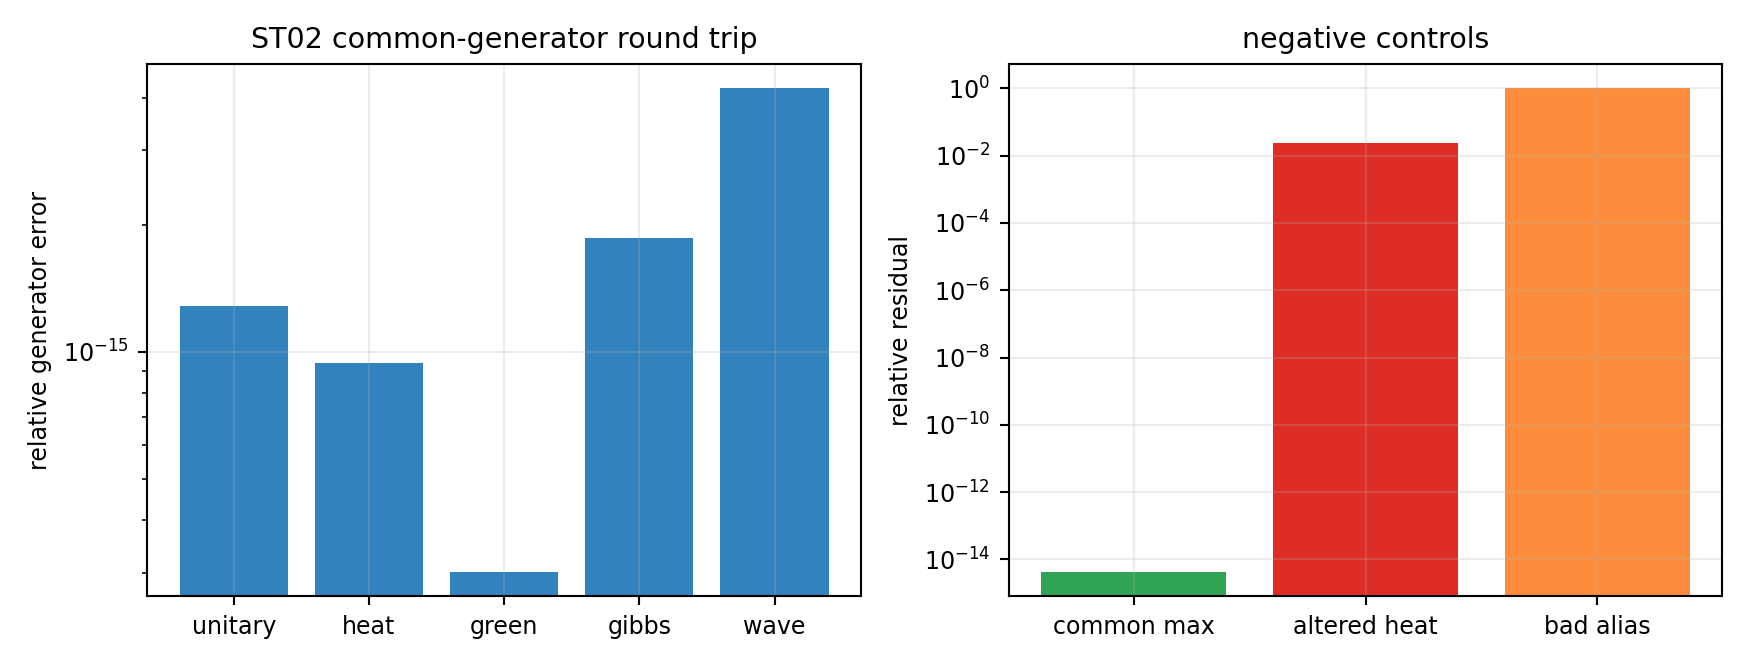
\includegraphics[width=0.92\textwidth]{FIN_ST01_ST15_Figures/st02_common_generator_and_controls.png}
\caption{Common-generator round trip and negative controls. The small errors validate the implementation; they are not independent tomography.}
\end{figure}

\subsection{No-refit cross-channel prediction}

ST13 calibrates $A$ from the heat channel alone. With no further fitting it predicts unitary, Green, Gibbs, and wave matrices with errors between $8.01\times10^{-16}$ and $1.55\times10^{-15}$. A unitary holdout generated from $A+0.08vv^T$ has error $0.010796$ and is rejected.

\boundary{} Both successes are closed-loop synthetic tests because the target channels were generated locally. They establish an executable falsifier for the narrow one-generator ansatz $H_{1A}$; they do not show that physical sectors share this $A$.

\section{ST03 --- A broader null atlas}

Five ensembles of $1{,}200$ matrices each were tested: positive radial circulant Laplacians, positive nonradial graph Laplacians, random PSD matrices with the uniform zero mode, isospectral rotations of strict, and signed radial kernels.

\begin{table}[H]
\centering
\small
\caption{ST03 ensemble summary.}
\begin{tabularx}{\textwidth}{@{}Xrrrr@{}}
\toprule
Ensemble & PSD rate & Markov/M rate & median dihedral residual & median kernel fingerprint\\
\midrule
positive radial & $1.000$ & $1.000$ & $3.32\times10^{-16}$ & $1.162$\\
positive nonradial graph & $1.000$ & $1.000$ & $0.236$ & $1.063$\\
random PSD, fixed zero mode & $1.000$ & $0.000$ & $0.516$ & $1.272$\\
isospectral rotations & $1.000$ & $0.000$ & $0.285$ & $1.086$\\
signed radial & $0.204$ & $0.015$ & $3.15\times10^{-16}$ & $2.444$\\
\bottomrule
\end{tabularx}
\normalsize
\end{table}

The isospectral ensemble preserves all twelve eigenvalues with maximum discrepancy $4.89\times10^{-15}$ while generically destroying dihedral and M-matrix structure.

\begin{theorem}[Isospectral identification obstruction]
Let $Q$ be any orthogonal transformation fixing the uniform zero mode. Then $QAQ^T$ has the same spectrum and all spectral trace invariants as $A$. Generic such $Q$ does not preserve the vertex algebra, dihedral action, or off-diagonal sign pattern. Therefore spectral data alone cannot identify the FIN vertex geometry or Markov interpretation.
\end{theorem}

The frozen kernel-law score is the coefficient of variation of
\[
\frac{(1+d^{1.8})w_d}{\cos(0.18575d+0.16250)},\qquad d=1,\ldots,6.
\]
It is $1.81\times10^{-16}$ for strict and at least $0.326$ in the positive-radial null sample. This is highly specific to the defining formula, but it is tautological as physics.

\begin{figure}[H]
\centering
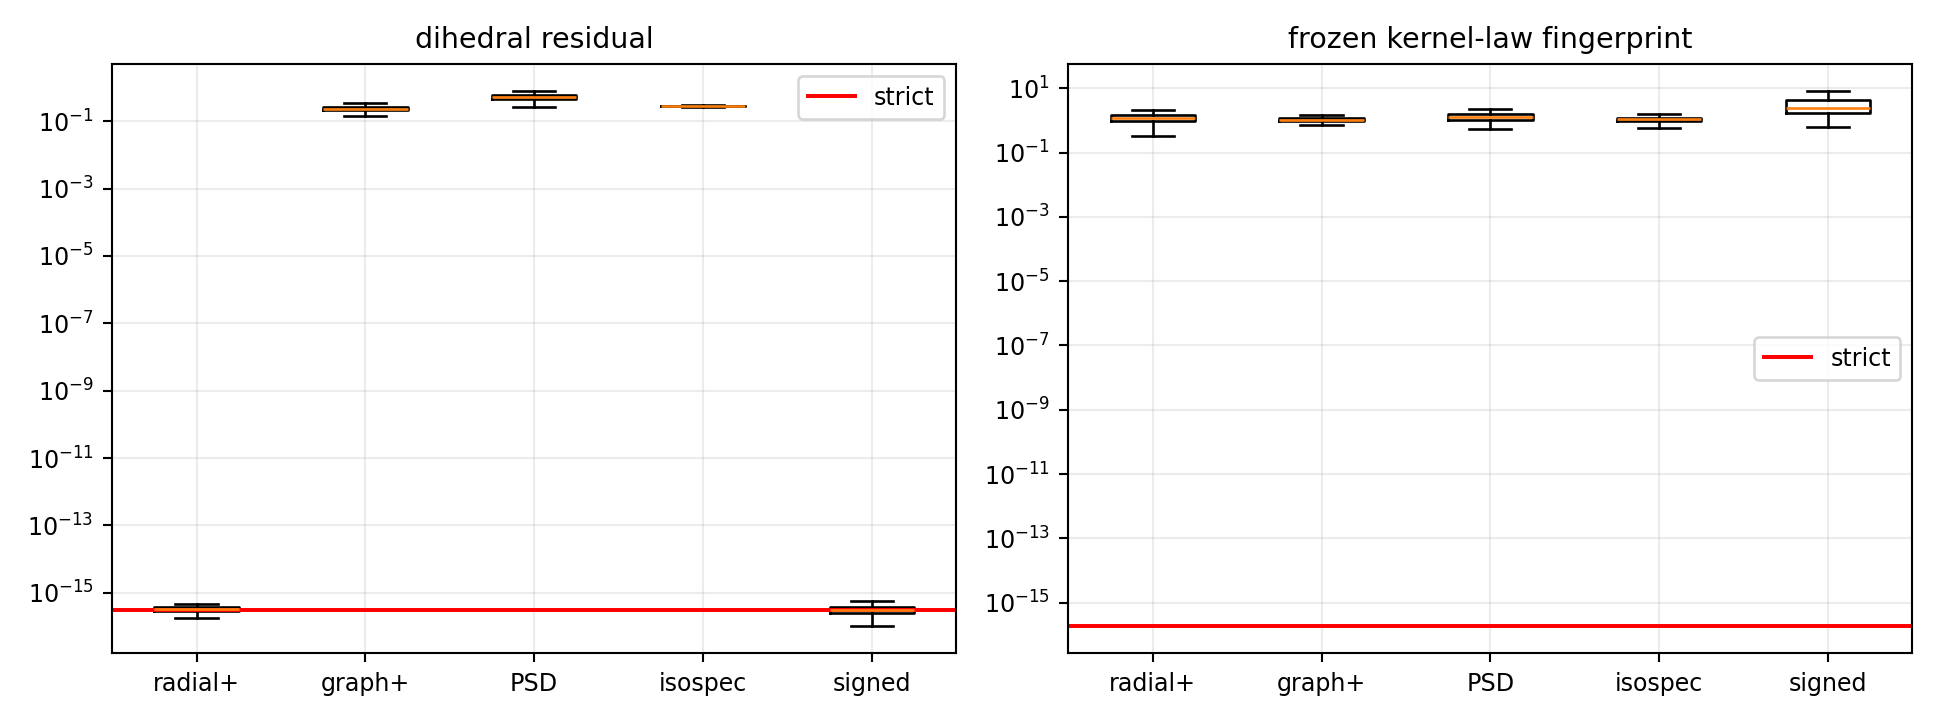
\includegraphics[width=0.94\textwidth]{FIN_ST01_ST15_Figures/st03_multiclass_null_atlas.png}
\caption{Symmetry and kernel-law fingerprints across five null classes. Exact kernel recognition is not a novel physical prediction.}
\end{figure}

\section{ST04 --- Minimal algebra completion and its selector cost}

The functional algebra generated by strict $A$ has dimension seven. Four closures were computed:
\[
\begin{array}{c|c}
\text{generators}&\dim\mathcal A_{\rm gen}\\\hline
A&7\\
A,\ \operatorname{diag}(0,1,\ldots,11)&144\\
A,\ \operatorname{diag}(d(x,0))&74\\
A,\ i(S-S^T)&12.
\end{array}
\]

\begin{theorem}[Conditional one-generator completion]
Let $B$ be diagonal with twelve distinct entries. Any matrix commuting with $B$ is diagonal. Since every off-diagonal entry of strict $A$ is nonzero, a diagonal matrix commuting with $A$ must be scalar. Thus the joint commutant of $A$ and $B$ is scalar, and the finite-dimensional Burnside theorem gives
\[
C^*(A,B)=M_{12}(\mathbb C).
\]
One extra generator is sufficient and necessary because $C^*(A)\ne M_{12}(\mathbb C)$.
\end{theorem}

The theorem does not solve QW-2191. $B=\operatorname{diag}(0,\ldots,11)$ explicitly supplies labels and orientation. The anchored distance observable supplies a preferred vertex but preserves one reflection, explaining dimension $74$. The chiral circulant breaks reflection but commutes in Fourier space and reaches only dimension $12$.

\section{ST05 --- Continuum nonidentifiability}

Two explicit families agree exactly with strict at $N=12$:
\begin{enumerate}
\item a fixed lattice-range family retaining $w_1,\ldots,w_6$ and setting all longer weights to zero;
\item a dense family evaluating the profile at the scaled distance $12d/N$ and renormalizing its row sum to $s$.
\end{enumerate}

\begin{table}[H]
\centering
\caption{First positive eigenvalue for two continuations.}
\begin{tabular}{@{}rrrr@{}}
\toprule
$N$ & fixed lattice range & scaled dense & direct integer extension Markov?\\
\midrule
12 & $0.754121$ & $0.754121$ & yes\\
24 & $0.241986$ & $0.593359$ & no\\
48 & $0.064108$ & $0.532680$ & no\\
96 & $0.016264$ & $0.506480$ & no\\
192 & $0.004081$ & $0.494274$ & no\\
\bottomrule
\end{tabular}
\end{table}

The fitted gap exponents are $-1.96485$ and $-0.08635$. They imply incompatible continuum scalings. A third, literal integer-distance extension first has a negative weight at $d=8$; it loses the Markov generator property and becomes non-PSD in the tested family from $N=48$.

\begin{theorem}[Finite-endpoint nonidentifiability]
A single matrix $A_{12}$ cannot determine a unique refinement sequence. Infinitely many families can be defined to equal $A_{12}$ at $N=12$ and differ for all larger $N$. Therefore QFT, GR, heat-kernel asymptotics, dimension, and locality cannot be derived from the endpoint without an additional canonical refinement principle.
\end{theorem}

\begin{figure}[H]
\centering
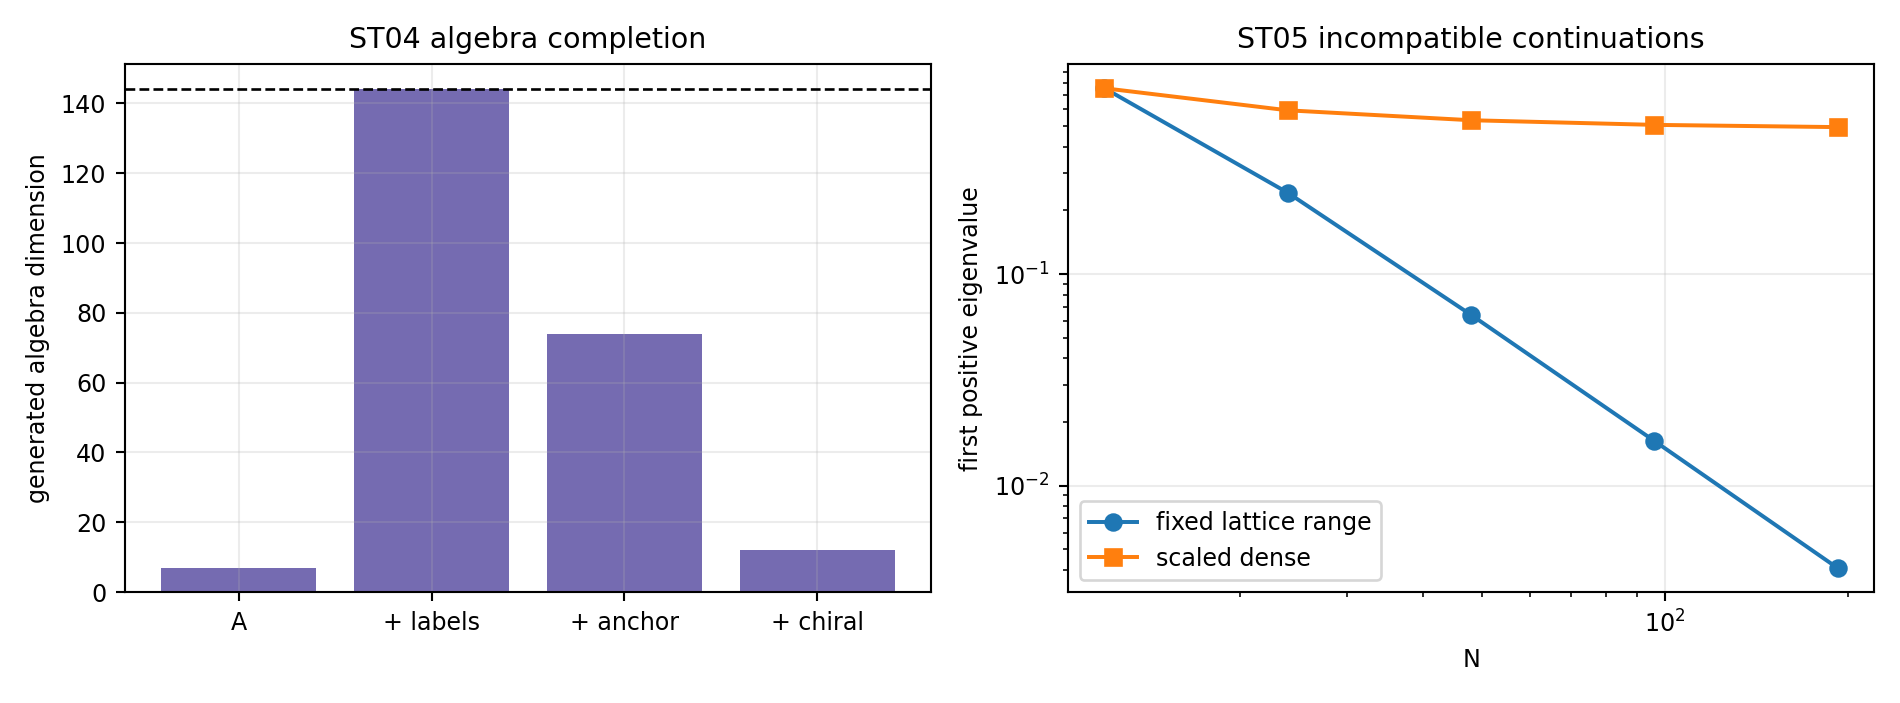
\includegraphics[width=0.93\textwidth]{FIN_ST01_ST15_Figures/st04_algebra_st05_continuum.png}
\caption{Left: algebra completion. Right: incompatible gap scaling for two equally admissible continuations.}
\end{figure}

\section{ST06 --- Lorentzian and propagation audit}

For $x\ne y$,
\[
\left.\frac{d}{dt}e^{-itA}_{xy}\right|_{t=0}=-iA_{xy}=iW_{xy},\qquad
\left.\frac{d}{dt}e^{-tA}_{xy}\right|_{t=0}=-A_{xy}=W_{xy}.
\]
Moreover,
\[
\cos(t\sqrt A)_{xy}=-\frac{t^2}{2}A_{xy}+O(t^4).
\]
Because strict $W_{xy}$ is nonzero at every cyclic distance, coherent, heat, and wave channels all develop direct remote tails. At $t=10^{-3}$ the strict unitary probability outside radius one is $9.62\times10^{-8}$, versus $2.44\times10^{-14}$ for a nearest-neighbor control. The strict heat mass is $7.20\times10^{-4}$ versus $2.21\times10^{-7}$.

\begin{theorem}[No exact nontrivial cyclic cone]
The frozen strict operator cannot satisfy an exact propagation cone based on the original cyclic distance: every remote pair is coupled in the first derivative of the unitary and heat semigroups and in the second derivative of the wave propagator.
\end{theorem}

The nearest-neighbor finite graph also has analytic tails at higher order, so exact finite propagation is not recovered merely by truncation. A Lorentzian limit would require a refinement theorem, a scale-dependent bound, and a vanishing exterior tail.

\begin{figure}[H]
\centering
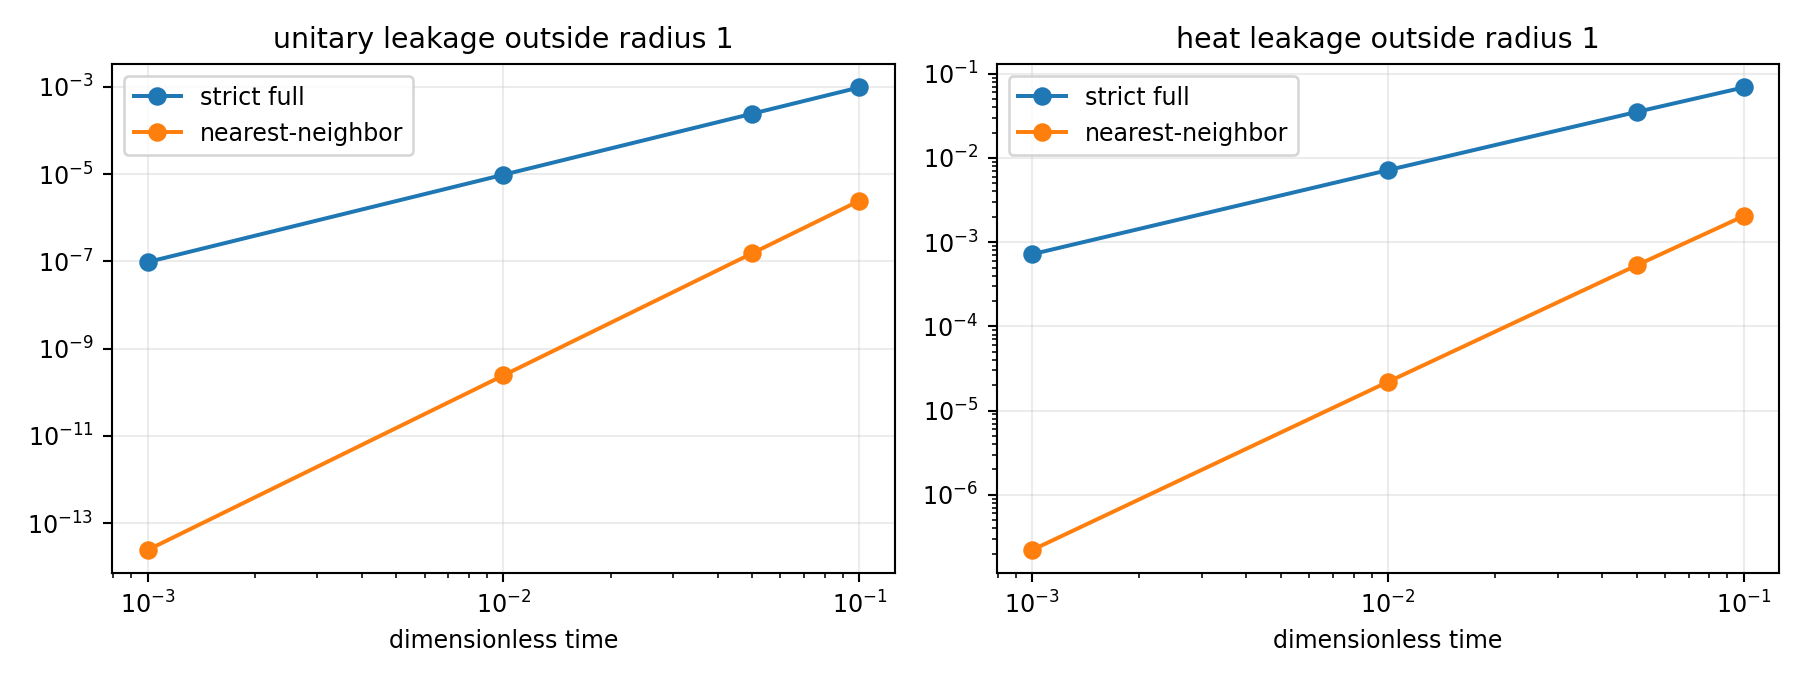
\includegraphics[width=0.91\textwidth]{FIN_ST01_ST15_Figures/st06_propagation_leakage.png}
\caption{Remote leakage for strict and a nearest-neighbor control. Full strict coupling removes even the path-order suppression present in the local control.}
\end{figure}

\section{ST07 --- Information to thermodynamics}

Let
\[
\gamma=\frac{e^{-\beta H}}{Z},\qquad
S(\rho)=-\operatorname{tr}(\rho\log\rho),\qquad
F_\beta(\rho)=\operatorname{tr}(\rho H)-\beta^{-1}S(\rho).
\]
Then
\[
D(\rho\|\gamma)=\operatorname{tr}\rho(\log\rho-\log\gamma)
=\beta\bigl(F_\beta(\rho)-F_\beta(\gamma)\bigr).
\]
The noncommuting matrix replay error is $6.44\times10^{-15}$.

\begin{theorem}[Conditional information--free-energy bridge]
Relative entropy becomes a free-energy difference after a Hamiltonian and inverse bath temperature are supplied. The Gibbs state is invariant under
\[
H\mapsto cH,qquad \beta\mapsto\beta/c,
\]
so probabilities do not separately identify energy and temperature. A thermodynamic process additionally requires a process/instrument family, bath semantics, and an energy/action unit.
\end{theorem}

The minimal equilibrium semantics is $(\rho,H,\beta,E_*)$. The minimal process-level tuple is $(\rho,H,\beta,\mathcal P,E_*)$. Removing any entry respectively destroys state expectations, energy, thermal direction, the meaning of work, heat, or erasure, or dimensional calibration. FIN has not internally sourced these entries.

\section{ST08 --- Gauge and holonomy receiver}

An antisymmetric link phase $\theta_{xy}=-\theta_{yx}$ defines
\[
(W_\theta)_{xy}=W_{xy}e^{i\theta_{xy}},\qquad A_\theta=sI-W_\theta.
\]
For $G_\chi=\operatorname{diag}(e^{i\chi_x})$ and
\[
\theta'_{xy}=\theta_{xy}+\chi_x-\chi_y,
\]
one has
\[
A_{\theta'}=G_\chi A_\theta G_\chi^*.
\]
The numerical covariance residual is $6.25\times10^{-16}$. A nearest-cycle flux $\Phi=0.37$ has holonomy
\[
\mathcal W=\prod_{x=0}^{11}e^{i\theta_{x,x+1}},
\]
whose gauge residual is $3.89\times10^{-16}$. The discrete probability current satisfies its continuity identity to $6.67\times10^{-17}$.

\conditional{} This is a valid $U(1)$ receiver. It is not a derived gauge sector. The group, connection, and flux were inserted. No electric field, Gauss constraint, Ward hierarchy, or Yang--Mills dynamics follows from strict $A$.

\section{ST09 --- Coercive saturating mediator}

P527 generated an attractive quartic by eliminating a positive mediator, but the resulting local jet was not globally bounded. ST09 replaces the linear density coupling by
\[
q(\rho)=\frac{\rho}{1+\rho/R}
\]
and considers
\[
E(\psi,\chi)=\frac12\langle\psi,A\psi\rangle
+\sum_x\left[\frac b2\chi_x^2-g\chi_xq(\rho_x)+\frac\mu2\rho_x\right],
\qquad \rho_x=|\psi_x|^2.
\]
Stationary elimination gives
\[
\chi_x^*=\frac gbq(\rho_x),\qquad
E_{\rm eff}=\frac12\langle\psi,A\psi\rangle
-\frac{g^2}{2b}\sum_xq(\rho_x)^2+\frac\mu2\sum_x\rho_x.
\]
At small density,
\[
-\frac{g^2}{2b}\rho^2+\frac{g^2}{bR}\rho^3+O(\rho^4),
\]
so the attractive P527 fourth-order jet is retained and followed by positive saturation.

\begin{theorem}[Global coercivity]
For $b,g,R,\mu>0$,
\[
E_{\rm eff}(\psi)\ge \frac\mu2\|\psi\|^2-\frac{Ng^2R^2}{2b}.
\]
Hence $E_{\rm eff}$ is bounded below and coercive on the finite state space. For the illustrative choice $(b,g,R,\mu)=(1,1,2,0.15)$, the bound is $-24$, the sampled minimum is $-8.196$, and the energy at uniform amplitude $100$ is $726.1$.
\end{theorem}

\boundary{} The theorem constructs the missing global completion, but $q$, $R$, and $\mu$ are new axioms. It does not derive a FIN soliton or prove orbital stability.

\section{ST10 --- Hamiltonian memory and Krein audit}

The P530 Hamiltonian memory realization has a $96\times96$ linearization $J$. With the canonical block symplectic matrix $J_0$, ST10 reconstructs
\[
J=J_0L,qquad L=-J_0J=L^T
\]
with exactly zero floating symmetry residual for the implemented block formula. Across mediator speeds $0.6\le c\le2.6$, $L$ has one negative, 94 positive, and one neutral direction. Therefore the elementary sufficient theorem $L>0\Rightarrow\sigma(J)\subset i\mathbb R$ does not apply.

The scan finds 17 unstable and 34 numerically stable samples, with a transition bracket $[1.24,1.28]$. At $c=1.60$, all 47 positive-imaginary sampled modes have positive nonzero Krein form; the minimum absolute form is $0.00571$. The unit-scale relaxation realization has spectral abscissa $0.67278$.

\begin{figure}[H]
\centering
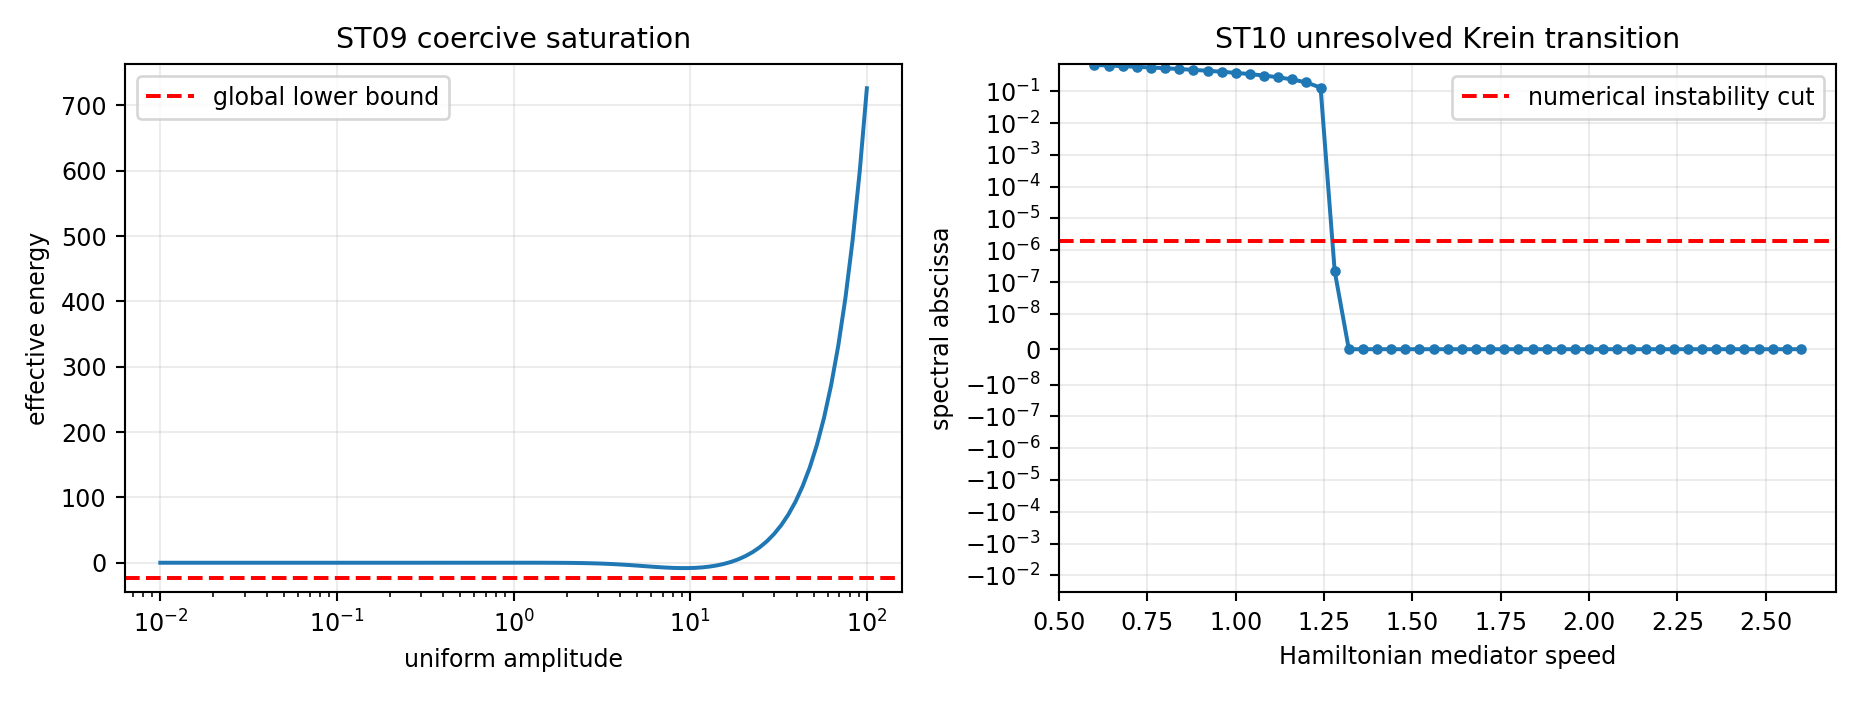
\includegraphics[width=0.93\textwidth]{FIN_ST01_ST15_Figures/st09_saturation_st10_memory.png}
\caption{Left: the constructed coercive energy. Right: the numerical Hamiltonian-memory transition.}
\end{figure}

\failed{} The scan does not prove an exact transition, exclude a zero-frequency collision, or establish global Krein stability. It sharpens the target: an exact treatment must quotient the neutral gauge mode, isolate the single negative direction, and certify the collision mechanism.

\section{ST11 --- Schur reduction versus RG}

For a positive block matrix $M$ and disjoint hidden sets $H_1,H_2$, exact elimination is associative:
\[
\operatorname{Schur}_{H_2}\bigl(\operatorname{Schur}_{H_1}(M)\bigr)
=\operatorname{Schur}_{H_1\cup H_2}(M).
\]
Using $M=A+0.4I$, retaining vertices $\{0,3,6,9\}$, and reversing two four-vertex elimination blocks gives maximum difference $3.41\times10^{-16}$.

After each first stage, setting off-diagonal entries below $0.08$ to zero produces a relative order dependence of $0.007821$. Thus exact Gaussian marginalization is scheme independent, but an approximation/projection rule restores scheme dependence.

\begin{figure}[H]
\centering
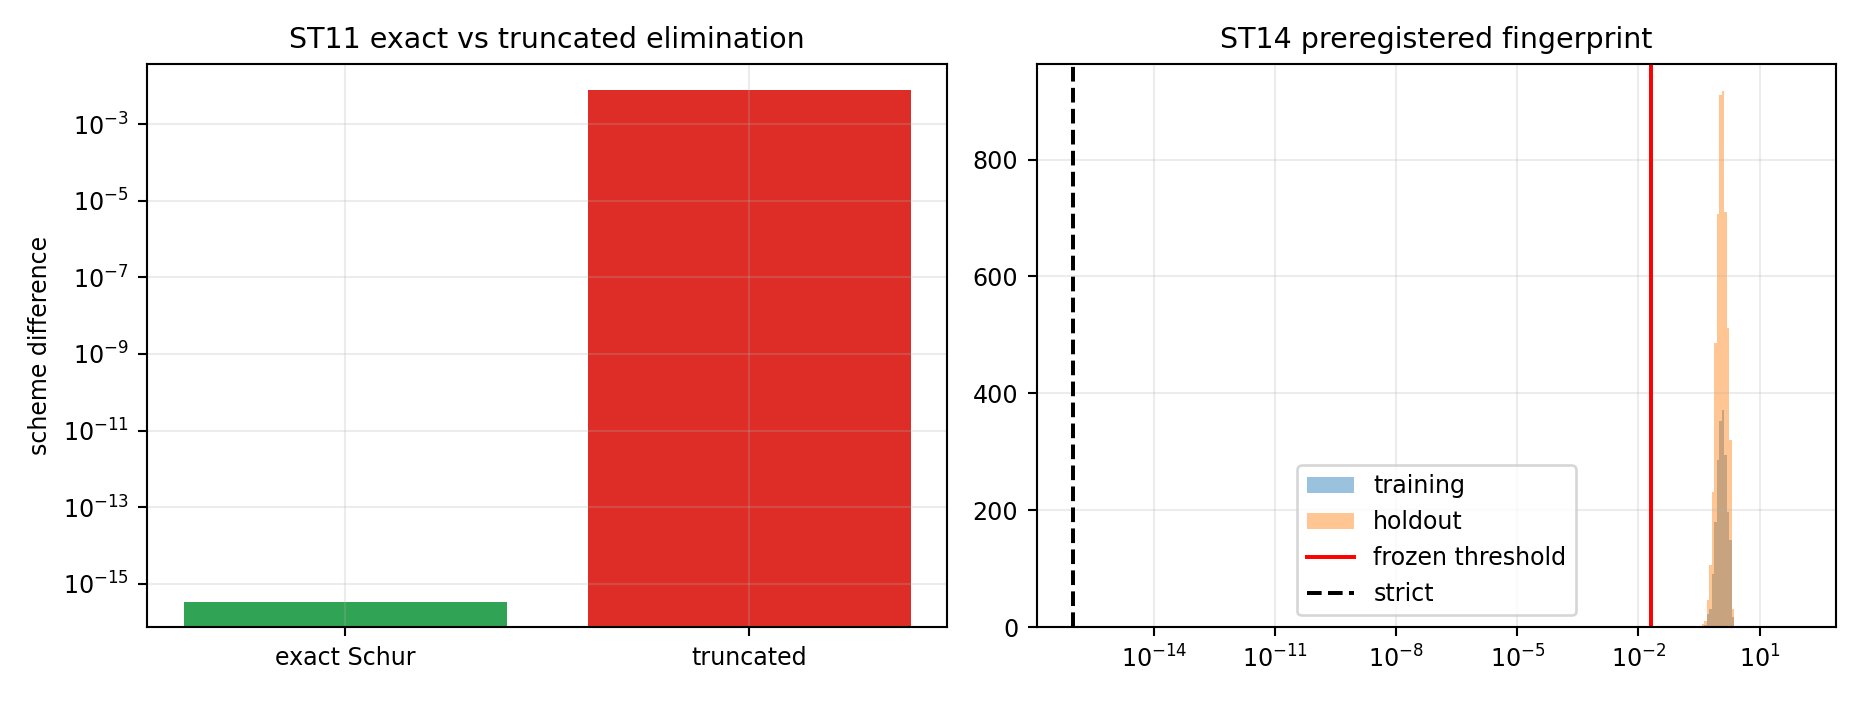
\includegraphics[width=0.93\textwidth]{FIN_ST01_ST15_Figures/st11_rg_st14_prediction.png}
\caption{Left: exact and truncated elimination order dependence. Right: the ST14 frozen fingerprint holdout.}
\end{figure}

\boundary{} Associativity is not a renormalization-group fixed point. FIN still lacks a canonical $N\to\infty$ family, scale parameter, coupling flow, universal exponent, and scheme-independent continuum observables.

\section{ST12 --- Legacy-to-strict physical-role gate}

The historical legacy formulas give
\[
\frac{\alpha_{\rm geo}}{12}=0.2310490602,qquad
\frac{\alpha_{\rm geo}}{2\beta_{\rm tors}}(1-\beta_{\rm tors})=137.2431418
\]
for $\alpha_{\rm geo}=4\ln2$ and $\beta_{\rm tors}=0.01$. These numerical values remain historical identities, not strict predictions.

\begin{table}[H]
\centering
\small
\caption{ST12 role-transfer gate.}
\begin{tabularx}{\textwidth}{@{}p{0.29\textwidth}p{0.18\textwidth}X@{}}
\toprule
Historical role & Value & Current verdict\\
\midrule
weak-mixing expression & $0.231049$ & blocked: no completion or role-transfer theorem\\
electromagnetic inverse expression & $137.243142$ & blocked: no completion or role-transfer theorem\\
$\beta^N$ gravity hierarchy & --- & blocked: no dimensional/role theorem\\
phase/orientation selector & --- & refuted inside Aut$(\mathbb Z_{12})$-invariant functional calculus\\
$\alpha_{\rm geo}$ information normalization & $2.772589$ & numerical identity only; no strict transfer\\
\bottomrule
\end{tabularx}
\normalsize
\end{table}

The completion endpoint, typed strict additions, and role-invariance theorem are all absent. The requested downstream role audit is therefore not admissible. This is a gate result, not a rejection of every possible future completion.

\section{ST14 --- Hashed prediction ledger}

After a $2{,}000$-sample training calculation, the kernel-law score and threshold $0.02$ were serialized and hashed before generating a separate $5{,}000$-sample holdout. The preregistration hash is
\begin{center}
\texttt{2f16938bd05d50a8767ad76e7a9e0acaeff95f474216bd5be8426017e4c3e76a}.
\end{center}
Strict has score zero to floating precision. The minimum holdout score is $0.262116$ and no sample passes the frozen threshold. Conditional on the declared lognormal measure, the exact one-sided $95\%$ upper rate after zero events is $5.99\times10^{-4}$.

\failed{} This does not qualify as a new physical prediction. The score directly tests the analytic formula used to define strict. It is valuable for implementation integrity and custody practice only. Moreover, provider, registrar, and analyst are the same local workflow; independent custody is absent.

\section{ST15 --- Formal-core replay}

The formal certificate checks:
\begin{enumerate}
\item the symbolic Dirichlet identity for arbitrary symmetric three-vertex weights;
\item an exact rational Schur/inverse-block identity;
\item symbolic invariance of $\beta E$ under $(E,\beta)\mapsto(cE,\beta/c)$;
\item the Aut$(\mathbb Z_{12})$ unit orbit $\{1,5,7,11\}$ containing both $+1$ and $-1$;
\item strict translation/reflection residual below $10^{-12}$;
\item the seven-dimensional functional algebra result.
\end{enumerate}
All six checks pass. The strict symmetry residual is $6.28\times10^{-16}$.

\boundary{} SymPy proves the declared symbolic and rational identities, while strict-kernel checks use binary64 arithmetic and rank tolerances. The package is not proof-assistant machine checking.

\section{What theoretical objects were actually constructed?}

The batch constructs four reusable objects:
\begin{enumerate}
\item the \textbf{Typed Physical-Shadow Certificate} of ST01;
\item the \textbf{Frozen Common-Generator Falsifier} of ST02/ST13;
\item the \textbf{Inserted $U(1)$ Link Receiver} of ST08;
\item the \textbf{Coercive Saturating-Mediator Completion} of ST09.
\end{enumerate}

Only the first two are neutral audit machinery. The latter two are conditional theory extensions. They show that gauge covariance and a globally stable attractive response can be constructed compatibly with the finite strict operator. They do not show that strict FIN generates either construction.

The minimal operational target remains a typed system of the form
\[
\mathfrak F=(\mathcal A,\mathcal H,A,E_A,\Omega,\Phi,\mathcal C,\mathcal U,
\mathcal S,\mathcal P,\mathcal E,\mathfrak I,\mathfrak M,\boxtimes,\mathcal R),
\]
containing observables, states, dynamics, contexts/refinements, units/clock, sectors, preparations, environment, instruments, apparatus/calibration, composition, and record.

\section{Was the single missing theorem found?}

No. The attempted single-theorem closure separates into at least five independent obligations:
\begin{enumerate}
\item \textbf{algebra/selector:} ST04 can complete the algebra only by adding a label-bearing observable;
\item \textbf{dimensions:} ST07 proves a scale orbit rather than selecting energy, temperature, or action;
\item \textbf{refinement:} ST05 proves that $A_{12}$ does not determine a unique continuum family;
\item \textbf{locality/causality:} ST06 excludes an exact nontrivial cyclic cone for frozen strict;
\item \textbf{operations/evidence:} ST01 and ST14 leave apparatus, independent custody, and external record ungenerated.
\end{enumerate}

\resultbox{\textbf{Deepest surviving interpretation.} The current strict FIN object is a finite information-spectral generator with several exact mathematical transforms and useful conditional extensions. It is not yet a physical substrate theorem. The missing bridge is not one equation but a typed operational-refinement structure whose components are independently necessary.}

\section{Recommended Programs ST16--ST27}

\begin{longtable}{@{}p{0.08\textwidth}p{0.11\textwidth}p{0.70\textwidth}@{}}
\toprule
ID & Priority & Study and success criterion\\
\midrule
ST16 & 1 & Exact Krein/zero-mode certificate for the P530 Hamiltonian memory family; isolate or refute the sampled transition.\\
ST17 & 2 & Selector-free algebra candidates; prove a strict no-go if every Aut$(\mathbb Z_{12})$-natural generator remains reducible.\\
ST18 & 3 & Derive a FIN-internal refinement functor rather than choosing either ST05 continuation.\\
ST19 & 4 & Replace the definitional ST14 fingerprint with a derived preregistered cross-sector observable.\\
ST20 & 5 & Interval-enclose the ST02 matrix logarithms, inverse branches, projector matching, and altered-channel separation.\\
ST21 & 6 & Establish approximate Lieb--Robinson-type bounds for truncated or decaying FIN$_N$ candidates.\\
ST22 & 7 & Prove minimality or redundancy of every component in the ST01 operational tuple.\\
ST23 & 8 & Derive a connection from a new strict-sourced object or certify that every ST08-type gauge receiver is inserted.\\
ST24 & 9 & Classify all globally coercive saturations sharing the P527 fourth-order jet and compare their universality.\\
ST25 & 10 & Port ST15 to a pinned proof-assistant toolchain and remove the binary64/rank trust boundary.\\
ST26 & 11 & Build one dimensional-equivariance theorem covering unitary, wave, heat, Green, and Gibbs sectors.\\
ST27 & 12 & Construct adversarial sector-specific refits that mimic $H_{1A}$ and prove the frozen protocol rejects them.\\
\bottomrule
\end{longtable}

\section{Final verdict}

The fifteen programs materially sharpen the theory.

\begin{itemize}
\item The common spectral family is reproducible and falsifiable, but generic spectral facts are not FIN-specific.
\item Spectral information does not determine the vertex geometry, observable algebra, or continuum.
\item Full algebra, gauge covariance, thermodynamics, and global nonlinear coercivity can all be constructed, but each construction exposes the extra premise it needs.
\item Frozen strict is not locally causal in the original cyclic metric.
\item Legacy physical roles remain blocked from strict.
\item The only preregistered holdout passed in this batch is a kernel-definition fingerprint, not a physical prediction.
\end{itemize}

Consequently, ST01--ST15 do not establish FIN as a Theory of Everything. They replace an undifferentiated ``physics gap'' by a finite list of typed mathematical obligations, construct one viable nonlinear completion, and prove several no-go results that prevent future work from mistaking spectral resemblance for physical derivation.

\appendix
\section{Reproduction}

\begin{verbatim}
MPLCONFIGDIR=/tmp/fin-st-mpl python3 fin_st01_st15_research.py
MPLCONFIGDIR=/tmp/fin-st-test-mpl \
  python3 -m unittest -v test_fin_st01_st15.py
pdflatex -interaction=nonstopmode -halt-on-error \
  FIN_ST01_ST15_Shadow_to_Physics_Bridge_Research_Report_EN.tex
sha256sum -c FIN_ST01_ST15_RELEASE_MANIFEST.sha256
\end{verbatim}

The analysis writes deterministic JSON, CSV, six figures, a formal-core certificate, and the ST14 preregistration record. Seventeen acceptance tests pass.

\section{Internal provenance and trust boundaries}

ST09 continues the P527 auxiliary-field sign mechanism. ST10 uses the declared P530 Hamiltonian and relaxation memory realizations. Their upstream sources are:
\begin{itemize}
\item \texttt{FIN\_Programs\_527\_536\_Auxiliary\_Field\_Memory\_and\_Exact\_Replay\_Report\_EN.pdf};
\item \texttt{FIN\_Programs\_527\_536\_Results.json};
\item \texttt{RELEASE\_10\_53\_PROGRAMS\_527\_536\_AUXILIARY\_FIELD\_MEMORY\_EXACT\_REPLAY.md};
\item \texttt{FIN\_Hypothetical\_TOE\_Shadow\_Atlas\_Comparative\_Report\_PL.pdf} for the ST01--ST15 recommendations and their original scope.
\end{itemize}

The current report independently recomputes every numerical quantity it presents. Imported branch and memory constructors retain their upstream numerical trust boundaries. No laboratory data or external audit is added.

\section{Scope and non-claims}

This release does not discharge QW-2191, select canonical orientation, derive a physical clock or absolute units, construct a unique continuum, complete the legacy-to-strict bridge, transfer any legacy physical role, prove a Standard Model or gravitational sector, provide apparatus, create independent custody, or establish a Theory of Everything.

\end{document}
